\section{Model}

%"
%==Model selection
%Model selection is the process of choosing an appropriate mathematical model
%from a class of models.
%" - Encyclopedia 

A whisker can be modeled as a function:

% In the following chapter we will formalize the whisker and discuss
% our model selection\cite{EncylopediaMachineLearning} process.

% First of we formalize the whisker by the definition

\begin{definition}
    Let 
    \begin{equation}
    \begin{split}
        \text{whisker} : \RR^+ &\rightarrow \RR^2 \\
                  \omega&\mapsto \text{whisker}(\omega)
    \end{split}
    \end{equation}
\end{definition}
where $\omega$ is a coordinate along the length of the whisker and
$\text{whisker}(\omega)$ is a point in the $x$-$y$ plane.

The tracking problem is then to find a function $\text{whisker}^*$
that approximates $\text{whisker}$. The function class used in a
model must satisfy the following conditions:

\begin{enumerate}
\item It must be able to approximate the whisker sufficiently
  well.

  \begin{example}
    A straight line will not suffice since the $\text{whisker}$ is
    generally curved and straight lines can not fill that partition of
    the space.
  \end{example}
  
\item The functions must be $C_1$ and be possible to represent with a
  finite number of parameters.
\end{enumerate}

With this in mind, two classes of functions immediately appear as
candidates:
\begin{itemize}
\item Polynomials $\sum_{i=0}^{n} a_i\omega^i$
\item Fourier series $\sum_{k=0}^{n} a_k\sin(\frac{k\pi\omega}{L}) +
  b_k\cos(\frac{k\pi\omega}{L})$
\end{itemize}

A brief analysis of both will follow, after a discussion of
simplifications and difference measures..

\subsection{Simplifications}
One simplification one might make is to assume that the root of the
whisker is fixed in some point on the snout. This means that we can
let the whisker function be defined in a head-fixed coordinate system
for each whisker, with the root of the whisker at the origin. This
gives us the boundary condition
\begin{equation}
    \label{eq:bv_root}
    \text{whisker}^*(0)=\bar{0}.
\end{equation}

Manual inspection of whisker videos suggests that this is not the case
for real whiskers. However, there seems to be some point within the
snouts that stays approximately still and can be regarded as the root
of the whisker. A better model could take this into account, but that
will not be covered in this thesis.

The thickness of a whisker is not constant, but decreases as the
distance from the head increases. A simple model for this is to define
the whisker thickness as

\begin{equation}
    d(\omega) = \begin{cases}
        D-\frac{D\omega}{L},~& \omega<L\\
        0,~& \omega\ge L
    \end{cases}
\end{equation}

where $D>0$ is the thickness at the root and $L>0$ is the total length of the
whisker.

\subsection{Difference measure}
The standard way to quantify distance between functions defined on an
interval $\interval{a}{b}$ is to use the norm in the
$\Lp[2](\interval{a}{b}, 1)$ Hilbert space. In this thesis, the norms
for $p = 2, 4, 8$ will be used, and the impact of the choice of $p$
will be investigated. This means that condition 1 above says the model
must be such that the $\Lp$ distance $\Lpnorm{\text{whisker} -
  \text{whisker*}}$ can be made sufficiently small.

\subsection{Polynomial $\Spline{\omega}$}
The first and simplest candidate is the polynomials. Manual tests in
MATLAB indicate that three terms are enough to approximate a whisker
well enough that the difference is not visible to the naked eye. A
whisker function can therefore be modeled as a third degree polynomial
$\Spline{\omega}$, also known as a \emph{spline}.

These define parameterized curves in the $xy$ plane as
\begin{equation}
  (\omega,\Spline{\omega})
\end{equation}

This choice can be justified by comparing with the theory of beams
under small deformations in solid mechanics. After all, a whisker is
not too different from a beam. The two main assumptions for this to
hold is that deformations are small and that the effects of motion on
whisker deformation are negligible. \cite{Hallfasthet} This may not
quite be the case, but a spline is still capable of approximating the
momentaneous shape of a whisker well enough.

\subsection{Sine series $\sum a_k\sin \left(\frac{k\pi\omega}{L}\right)$}
Another promising candidate is the Fourier series. Considering
\eqref{eq:bv_root}, the Fourier series is reduced to a sine series
$\sum a_k\sin \left(\frac{k\pi\omega}{L}\right)$. However, such a
series will always be zero at $\omega = L$, and is therefore not a
reasonable model for whiskers. To address this, one could instead use
quarter-periods: $\sum a_k \sin\left( \frac{k\pi\omega}{2L}\right)$,
but at the cost of losing the orthogonality property of the sine
basis. Manual tests in MATLAB indicate that such a series to third
order performs approximately the same as a spline.

These define parameterized curves in the $xy$ plane as
\begin{equation}
    (\omega,\sum{a_n\sin (\frac{2\pi n}{L}\omega)})
\end{equation}


The choice of a sine series can be justified by comparing with the
theory of stiff strings in analytical mechanics. The movement equation
for a stiff string is a partial differential equation containing the
second and fourth spatial derivatives.\footnote{Source: Solving
  exercise 7.10 of \cite{VarKalk} using variational calculus.} A
classic separation of variables solution to the equation would be a
sine series for the spatial part.

\subsection{Theoretical evaluation}

It is hard to theoretically justify the choice of $\text{whisker}^*$
model since we do not have an analytic model for the $\text{whisker}$.

\begin{figure}
  \centering
  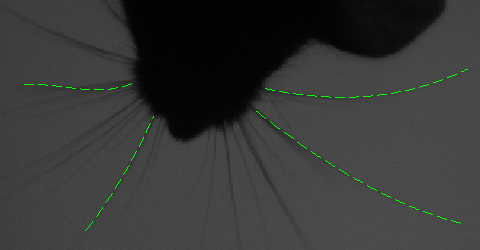
\includegraphics[width=0.45\textwidth]{rat-splines.png}
  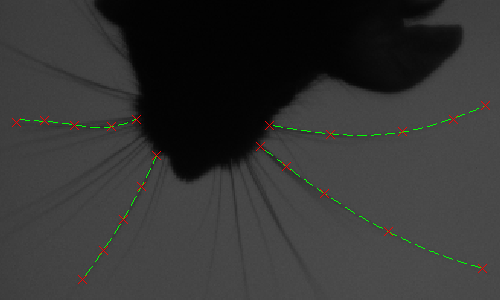
\includegraphics[width=0.45\textwidth]{rat-sines.png}
  \caption{Comparison of whisker models. Left: Splines, Right: Sine series}
  \label{fig:model-comparison}
\end{figure}

For this thesis, the spline model was used in the tracking engine. The
main reason for this is that it is slightly simpler than the sine
model. It also is rather easy to get an intuitive grasp of how the
parameters affect the curve shape - the $\omega^3$ term mostly affects
the tip of the whisker while the $\omega$ term affects the overall
orientation.
